\subsubsection*{Problem definition}

The aim of this example is to simulate the solute transport in an aquifer by convection with the influence of retardation as a result of sorption. Additionally, the transported mass will be degraded. The calculation area and boundary conditions are the same as described in chapter \ref{sec:decay}.


\textsl{Assumptions}

\begin{tabbing}
Component: \= linear sorption, decay \\
Aquifer: \> homogeneous, saturated, stationary flow \\
\end{tabbing}

\subsubsection*{Model set-up of the 1~D numerical model}

See chapter \ref{sec:decay}

The soil parameters are the same as listed in table \ref{tab51}. The decay rate $\lambda$ is 2$\cdot 10^{-7}$~s$^-1$. For the different simulation runs the Henry sorption coefficients are varied as listed in table \ref{tab52} to evaluate again the influence of sorption on mass transport.

\subsubsection*{Evaluation method}
The concentration distribution at a special point in time and over a given distance is calculated by equation \ref{eq53}. The analytical solutions are depicted in figure \ref{fig58} as single symbols.

\subsubsection*{Results}

The influence of radioactive decay on the transport process can be recognised at the typical declining exponential curves in figure \ref{fig58}. According to the different sorption coefficients the transport is retarded. Obviously, the numerical results (lines) meet well the analytical solutions. Therefore, it can be summarised that the transport under the combined consideration of both decay and sorption can be reproduced by the simulation with RockFlow.

\begin{figure}[htbp]
\centering
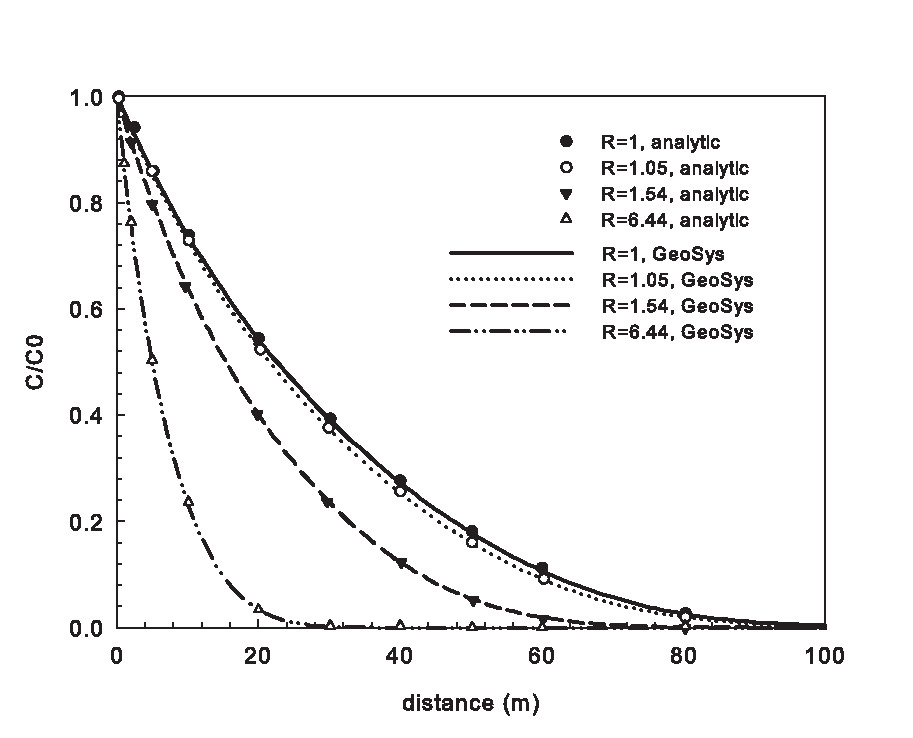
\includegraphics[width=0.8\textwidth]{C/figures/fig58.EPS}
\caption{Concentration distributions after 100~d (sorption and decay)}
\label{fig58}
\end{figure}

\begin{tabular}{|l|l|l|}
\hline
Benchmark & Problem type	& Path in benchmark deposit \\
\hline	
hc\_decay\_sorp\_henry\_1Du	& HC	& benchmarks $\backslash$HC$\backslash$sorption\_decay \\
\hline	
\end{tabular}
